\documentclass[a4paper, 10pt, fleqn]{article}
\usepackage[utf8]{inputenc}
\usepackage[T1]{fontenc}
\usepackage{textcomp}
\usepackage{lmodern}
\usepackage[ngerman]{babel}
\usepackage{enumerate}
\usepackage{xcolor}

\usepackage{amsmath}
\usepackage{graphicx}
\usepackage{geometry}
\usepackage{scrpage2}
\usepackage{lastpage}
\usepackage[hyphens]{url}
\usepackage{hyperref}
\usepackage{listings}
\usepackage{array}
\usepackage{subcaption}

\lstset{language=[ansi]C++}

\geometry{left=3cm, top=3cm, bottom=3cm, right=3cm}

\hypersetup{
    colorlinks,
    linkcolor={red!50!black},
    citecolor={blue!50!black},
    urlcolor={blue!80!black}
}

\pagestyle{scrheadings}
\ihead{PREN1 Gruppe 39}\ohead{Konzeptvarianten} 
\ifoot{\today} \ofoot{Seite \thepage\ von \pageref{LastPage}}
\newcolumntype{M}[1]{>{\centering\arraybackslash}m{#1}}

\begin{document}
\input{titlepageTR.tex}

\begin{figure}[h!]%Position festigen
\centering
\includegraphics[width=1.0\textwidth]{fig/morphologischeKasten_mitKonzeptvarianten.png}
\caption{Morphologischer Kasten}
\label{fig:Morphologischer Kasten}
\end{figure}


\clearpage
% !TEX root = ../Dokumentation.tex
\subsection{Chassis}

\textbf{Funktionsbeschrieb}
\textbf{Komponentenbeschrieb}
\textbf{Begründung}
Wenn benötigt
\textbf{Berechnungen}
\textbf{Testergebnisse}

% !TEX root = ../Dokumentation.tex
\subsection{Lenkung}

\textbf{Funktionsbeschrieb}
\\[0.2cm]
Die Lenkung ist eine Achsschenkellenkung. Sie wird heute in fast allen PKWs, LKWs, Omnibussen und sonstigen Nutzfahrzeugen eingesetzt. Bei dieser Art der Lenkung befinden sich die Räder auf einzelnen lenkbaren Achsschenkeln, die jeweils mit einem Spurstangenhebel versehen sind. Die Spurstangenhebel sind ungefähr senkrecht zur Vorderachse bzw. ungefähr parallel zur Längsachse des Fahrzeugs ausgerichtet und mittels einer Spurstange miteinander verbunden. Dadurch werden beide Räder gleichzeitig gelenkt.\\[0.2cm]
\textbf{Komponentenbeschrieb}
\\[0.2cm]
Mit einem Servomotor wird über eine Kegelradverbindung der Lenkschubhebel angetrieben. Dieser treibt wiederum die Spurstange an, welche die Bewegung über die Spurstangenhebel an die Räder weitergibt.
\begin{figure}[H]%Position festigen
\centering
\includegraphics[width=1\textwidth]{03_Loesungskonzept/pictures/Achsschenkellenkung.png}
\caption{Konzept der Achsschenkellenkung}
\label{fig:activityRoute}
\end{figure}\flushleft
\textbf{Begründung}\\[0.2cm]
%Für die Bildverarbeitung ist das Lenken und konstante Ausgleichen der Fahrbahn und Fahrtgeschwindigkeit mit zwei Motoren, welche jeweils ein Rad antreiben Nachteil.%
Bei der Zweiradvariante wird ein starkes Ruckeln oder Vibrieren durch die Lenkregelung befürchtet. Dies hätte grosse Nachteile in der Bildauswertung. Darum ist das Lösungskonzept mit einer Achsschenkellenkung ausgestattet. Von der konstruktiven Seite ist die Achsschenkellenkung im Vergleich zwar aufwändiger, aber für die Aufgabenstellung besser geeignet. Das Ziel einen möglichst konstanten Abstand zum Trottoir der Fahrbahn zu halten, ist mit einer Achsschenkellenkung einfacher. Weitere Gründe, welche für die Achsschenkellenkung sprechen, wurden schon im Kapitel \glqq{Chassis}\grqq  erläutert.
Die Begründung für die Wahl des Servomotors ist, dass die Lenkung keine 360° Bewegungen durchführen muss. Zudem ist die Position des Servos leicht zu steuern, ohne das zusätzlich eine Regelung eingebaut werden müsste. \\[0.2cm]
\textbf{Berechnungen}\\[0.2cm]
Berechnung Drehmoment Servo Lenkung
\begin{itemize}
\item Gewichtskraft auf jedes Rad $Fg = frac{m*g}{4}$
\item Abstand $l = 30mm$
\item $M = 2\cdot Fg\cdot l = 0.37Nm$
\item Sicherheitsfaktor = 1.5 (da Beschleunigung- und Bremskräfte vernachlässigt werden)
\item $M = 0.37\cdot 1.5 = 0.555Nm = 55.5Ncm$
\end{itemize}

% !TEX root = morphkasten.tex

\section{Greifer}


%##############
\subsection{Greifer rund}
\begin{figure} [hbp]
	\centering
	\includegraphics[width=0.5\textwidth]{fig/Greifer_rund.png}
	\caption{runder Greifer}
\end{figure}


\begin{table}[h]
\begin{tabular}{p{0.5\textwidth} | p{0.5\textwidth}}


 \textbf{Vorteile} & \textbf{Nachteile} \\ \hline
	 
\begin{itemize}
\item 2 Auflagepunkte am Container
\item Mit Zahnradübersetzung ist das Schliessen/Öffnen mit einem Motor möglich
\item keine Sensoren nötig um Schliessvorgang zu bestätigen
\item Automatische Zentrierung
\end{itemize}

 
 &
 
\begin{itemize}
\item Auf beiden Seiten hohe bzw. 2 Greiferbacken nötig um Stabilität zu garantieren
\item wenig Platz um Motor zu befestigen
\end{itemize}

\end{tabular}
\end{table}

\begin{table}[h]
\begin{tabular}{p{0.5\textwidth}p{0.5\textwidth}}


 \textbf{Risiken} & \\ \hline
	 
\begin{itemize}
\item Breitenbegrenzung überschreiten wegen der Länge des Greifers
\end{itemize}

 
\end{tabular}
\end{table}

\pagebreak


%##############
\subsection{Greifer gerade}
\begin{figure} [hbp]
	\centering
	\includegraphics[width=0.5\textwidth]{fig/Greifer_gerade.png}
	\caption{gerader Greifer}
\end{figure}

\begin{table}[h]
\begin{tabular}{p{0.5\textwidth} | p{0.5\textwidth}}


 \textbf{Vorteile} & \textbf{Nachteile} \\ \hline
	 
\begin{itemize}
\item grosse Auflagefläche für Container
\item Mit Zahnradübersetzung nur ein Motor zum Schliessen/Öffnen nötig
\end{itemize}

 
 &
 
\begin{itemize}
\item sehr breiter Greifer bei unpräziser Positionierung nötig
\item aufwändige Führung
\item hohes Gewicht
\item wenig Platz für Motor
\end{itemize}

\end{tabular}
\end{table}

\begin{table}[h]
\begin{tabular}{p{0.5\textwidth}p{0.5\textwidth}}


 \textbf{Risiken} & \\ \hline
	 
\begin{itemize}
\item Stabilität des Greifer fraglich
\item Motorenüberlastung
\end{itemize}

 
\end{tabular}
\end{table}

\pagebreak

% !TEX root = morphkasten.tex

\section{Beladen}


%##############
\subsection{Arm ohne Knick}

\includegraphics[width=0.5\textwidth]{fig/Beladen_1.png}

\begin{table}[h]
\begin{tabular}{p{0.5\textwidth} | p{0.5\textwidth}}


 \textbf{Vorteile} & \textbf{Nachteile} \\ \hline
	 
\begin{itemize}
\item nur ein Motor nötig für die gesamte Funktion
\item simple Lösung
\item komplette Entladung ohne Probleme möglich
\end{itemize}

 
 &
 
\begin{itemize}
\item keine
\end{itemize}

\end{tabular}
\end{table}

\begin{table}[h]
\begin{tabular}{p{0.5\textwidth}p{0.5\textwidth}}


 \textbf{Risiken} & \\ \hline
	 
\begin{itemize}
\item Länge von Drehgelenk zu Greifer Ende muss optimal gewählt werden
\item zu hohe Motorbelastung
\end{itemize}
 
\end{tabular}
\end{table}

\pagebreak


%##############
\subsection{Knickarm}

\includegraphics[width=0.5\textwidth]{fig/Beladen_2.png}

\begin{table}[h]
\begin{tabular}{p{0.5\textwidth} | p{0.5\textwidth}}


 \textbf{Vorteile} & \textbf{Nachteile} \\ \hline
	 
\begin{itemize}
\item Kompakte Bauweise (weniger breit als vorherige Variante)
\item Entladung einfach möglich 
\end{itemize}

 
 &
 
\begin{itemize}
\item 2 Motoren notwendig
\item aufwändiger Bewegungsablauf
\end{itemize}

\end{tabular}
\end{table}

\begin{table}[h]
\begin{tabular}{p{0.5\textwidth}p{0.5\textwidth}}


 \textbf{Risiken} & \\ \hline
	 
\begin{itemize}
\item zu frühes knicken (Schüttgut landet nicht in Behälter) 
\end{itemize}
 
\end{tabular}
\end{table}

\pagebreak

% !TEX root = morphkasten.tex

\section{Lagerung}


%##############
\subsection{Behälter}

\begin{figure} [hbp]
	\centering
	\includegraphics[width=0.3\textwidth]{fig/Unbenannt-1.png}
	\caption{Auffangbehälter, Schüttgutfluss mit Pfeilen angezeigt}
\end{figure}

\begin{table}[h]
\begin{tabular}{p{0.5\textwidth} | p{0.5\textwidth}}


 \textbf{Vorteile} & \textbf{Nachteile} \\ \hline
	 
\begin{itemize}
\item Keine elektrischen Komponenten notwendig
\item Vorgegebener Weg des Schüttguts
\end{itemize}

 
 &
 
\begin{itemize}
\item Maximale Höhe wird ausgenutzt
\item Aufwendiges Bauteil
\end{itemize}

\end{tabular}
\end{table}

\begin{table}[h]
\begin{tabular}{p{0.5\textwidth}p{0.5\textwidth}}


 \textbf{Risiken} & \\ \hline
	 
\begin{itemize}
\item Verschütten
\end{itemize}

 
\end{tabular}
\end{table}

\pagebreak


% !TEX root = ../Dokumentation.tex
\subsection{Entladen}

\textbf{Funktionsbeschrieb}\\[0.2cm]
\begin{figure}[H]
\centering
\includegraphics[width=0.5\textwidth]{03_Loesungskonzept/pictures/Entladen_Schraegbehaelter.png}
\caption{Entladen}
\end{figure}\flushleft

Beim Entladevorgang fährt das Fahrzeug bis auf 20mm +/- 5mm an den Rand des Entsorgungsbecken. Anschliessend wird die Klappe gelöst und diese fällt auf den Rand des Entsorgungsbecken. Über die Klappe rutscht das Schüttgut in das Entsorgungsbecken. Nach erfolgter Abladung fährt das Fahrzeug kurz nach links, damit das ganze Fahrzeug im Zielbereich steht. Dabei hängt die Klappe nach unten.\\[0.2cm]

\textbf{Komponentenbeschrieb}\\[0.2cm]
Die Klappe besteht aus einem handelsüblichen Scharnier auf dem eine Platte aus Acrylglas befestigt ist.
Die Klappe wird von einem Servomotor gehalten.\\[0.2cm]

\textbf{Berechnungen}\\[0.2cm]
Die Berechnungen zum Servo Motor für die Klappe sind schon im Kapitel Beladen zu finden. 

% !TEX root = morphkasten.tex

\section{Antrieb}


%##############
\subsection{DC-Motor}

\begin{figure}[h!]%Position festigen
\centering
\includegraphics[width=0.5\textwidth]{fig/dcmotor.jpg}
\caption{NiMH (Quelle: http://www.mind.ilstu.edu/)}
\label{fig:Java}
\end{figure}

\begin{table}[h]
\begin{tabular}{p{0.5\textwidth} | p{0.5\textwidth}}


 \textbf{Vorteile} & \textbf{Nachteile} \\ \hline
	 
\begin{itemize}
\item Niedriger Anschaffungspreis
\item Simpel in der Handhabung
\item Gut geeignet für permantente Drehung
\end{itemize}

 
 &
 
\begin{itemize}
\item Extra Regelung notwendig
\item Nur bedingt präzise
\item Hohe Wärmeentwicklung
\end{itemize}

\end{tabular}
\end{table}

\begin{table}[h]
\begin{tabular}{p{0.5\textwidth}p{0.5\textwidth}}


 \textbf{Risiken} & \\ \hline
	 
\begin{itemize}
\item Könnte für exaktes Arbeiten (z.B sofortiges Bremsen) zu ungenau sein.
\end{itemize}

 
\end{tabular}
\end{table}

\pagebreak


%##############
\subsection{Schrittmotor}

\begin{figure}[h!]%Position festigen
\centering
\includegraphics[width=0.5\textwidth]{fig/schrittmotor.JPG}
\caption{NiMH (Quelle: http://www.pollin.de/shop/index.html)}
\label{fig:Java}
\end{figure}

\begin{table}[h]
\begin{tabular}{p{0.5\textwidth} | p{0.5\textwidth}}


 \textbf{Vorteile} & \textbf{Nachteile} \\ \hline
	 
\begin{itemize}
\item Niedriger Anschaffungspreis
\item Genaue Positionsrückmeldung ohne Sensoren
\item Exakte Drehung/Kontrolle
\end{itemize}

 
 &
 
\begin{itemize}
\item Hohe Wärmeentwicklung
\item Hohe Betriebsspannung
\end{itemize}

\end{tabular}
\end{table}

\begin{table}[h]
\begin{tabular}{p{0.5\textwidth}p{0.5\textwidth}}


 \textbf{Risiken} & \\ \hline
	 
\begin{itemize}
\item Könnte bei zu langem permanentem Gebrauch Schaden nehmen.
\end{itemize}

 
\end{tabular}
\end{table}

\pagebreak

%##############
\subsection{BLCD-Motor}

\begin{figure}[h!]%Position festigen
\centering
\includegraphics[width=0.5\textwidth]{fig/blcd.jpg}
\caption{NiMH (Quelle: http://www.ti.com/tool/hvbldcmtr)}
\label{fig:Java}
\end{figure}

\begin{table}[h]
\begin{tabular}{p{0.5\textwidth} | p{0.5\textwidth}}


 \textbf{Vorteile} & \textbf{Nachteile} \\ \hline
	 
\begin{itemize}
\item Niedriger Anschaffungspreis
\item Lange Lebensdauer
\item Hohe Drehzahlen möglich
\item Hoher Wirkungsgrad
\end{itemize}

 
 &
 
\begin{itemize}
\item Extra Regelung notwendig
\item Nur bedingt präzise
\end{itemize}

\end{tabular}
\end{table}

\begin{table}[h]
\begin{tabular}{p{0.5\textwidth}p{0.5\textwidth}}


 \textbf{Risiken} & \\ \hline
	 
\begin{itemize}
\item Könnte für exaktes Arbeiten (z.B sofortiges Bremsen) zu ungenau sein.
\end{itemize}

 
\end{tabular}
\end{table}

\pagebreak

% !TEX root = morphkasten.tex

\section{Motor Lenkung}


%##############
\subsection{DC-Motor}

Im Kapitel 7.1 wurde die Variante DC-Motor bereits beschrieben.


%##############
\subsection{Schrittmotor}
Im Kapitel 7.2 wurde die Variante Schrittmotor bereits beschrieben.

%##############
\subsection{BLDC-Motor}
Im Kapitel 7.3 wurde die Variante BLDC-Motor bereits beschrieben.

%##############
\subsection{Servo-Motor}

\begin{figure}[h!]%Position festigen
\centering
\includegraphics[width=0.5\textwidth]{fig/servo.jpg}
\caption{Servo-Motor (Quelle: http://www.sachsendreier.com/asw/clernen/servo/servo.html)}
\label{fig:Java}
\end{figure}

\begin{table}[h]
\begin{tabular}{p{0.5\textwidth} | p{0.5\textwidth}}


 \textbf{Vorteile} & \textbf{Nachteile} \\ \hline
	 
\begin{itemize}
\item Sehr präzise
\item Sehr hoher Wirkungsgrad
\end{itemize}

 
 &
 
\begin{itemize}
\item Komplexe Ansteuerung
\item Hoher Anschaffungspreis
\item Hat einen begrenzten Drehwinkel
\item Relativ empfindlich
\end{itemize}

\end{tabular}
\end{table}

\begin{table}[h]
\begin{tabular}{p{0.5\textwidth}p{0.5\textwidth}}


 \textbf{Risiken} & \\ \hline
	 
\begin{itemize}
\item Erhötes Risiko, dass der Motor bei Versuchen Schaden nimmt.
\end{itemize}

 
\end{tabular}
\end{table}

\pagebreak

% !TEX root = morphkasten.tex

\section{Motor Greifer}


%##############
\subsection{Schrittmotor}
Im Kapitel 7.2 wurde die Variante Schrittmotor bereits beschrieben.

%##############
\subsection{BLCD-Motor}
Im Kapitel 7.3 wurde die Variante BLCD-Motor bereits beschrieben.

%##############
\subsection{Servo-Motor}
Im Kapitel 8.4 wurde die Variante Servo-Motor bereits beschrieben.
\pagebreak

% !TEX root = ../Dokumentation.tex
\subsection{Energieversorgung}

\textbf{Funktionsbeschrieb}\\[0.2cm]
Das autonome Entsorgungsfahrzeug muss mit Energie versorgt werden. Dazu werden Akkumulatoren eingesetzt, welche das Gerät während dem gesamten Einsatz mit Strom versorgen. 
\\[0.2cm]
\textbf{Komponentenbeschrieb}\\[0.2cm]
\begin{figure}[h]
\centering
\includegraphics[width=0.5\textwidth]{03_Loesungskonzept/pictures/lipo.jpg}
\caption{2400 mA/h Lipo  (Quelle:http://www.conrad.ch/ce/)}	
\end{figure}\\[0.2cm]
Um Störungen, die z.B durch den erhöten Anlaufstrom der Motoren verursacht werden könnten, zu vermeiden, werden die intelligenten Systeme (Microcontroller, Mini-Computer,etc.)möglichst getrennt von den Motoren gespiesen. Dazu wird einerseits ein 11.1Volt Lithium-Polymer-Akkumulator für die Motoren und andererseits ein 7.4 Volt Lipo für die empfindlichen Systeme  verwendet. Die finale Evaluation der Kapazitäten ist noch nicht abgeschlossen. Die Resultate der aktuellen Berechnungen werden im Verlauf des Kaptiels noch erläutert.
 \\[0.2cm]
\textbf{Begründung}\\[0.2cm]
Die Entscheidung wird damit begründet, dass Lithium-Polymer-Akkumulatoren in einem vielfältigen Sortiment erhältlich sind und damit eine grosse Flexibilität bei der Auswahl ermöglichen. Somit würde sich die Suche nach einem Ersatz bei allfälligen Änderungen vereinfachen. Ausserdem weisen LiPo, im Vergleich zu anderen Akkumulatoren eine wesentlich kompaktere Bauform auf was entscheidend für die Auswahl war. \\[0.2cm]
\textbf{Berechnungen}\\[0.2cm]
Kapazitätenberechnungen:
\begin{itemize}
\item DC-Motor für den Antrieb:
\[
\frac{P*t}{U} -> \frac{73.98W*0.25h}{12V}= 1.54 Ah
\]
\item Servomotor für die Lenkung:
\[
\frac{P*t}{U} -> \frac{3.76W*0.25h}{4.8V}= 0.19 Ah
\]
\item Servomotor für den Arm:
\[
\frac{P*t}{U} -> \frac{2.5W*0.25h}{4.8V}= 0.13 Ah
\]
\item Servomotoren für Kamerabewegung, Greifer und Behälteröffnung:
\[
\frac{P*t}{U} -> \frac{0.814W*0.25h}{4.8V}= 0.042 Ah
\]
\item Mini-Computer:
\[
I*t -> 2A+0.25h = 0.5 Ah
\]
\item Gesamtkapazität:
\[
1.54Ah+0.19Ah+0.13Ah+3*0.042Ah+0.5Ah = 2.53Ah
\]

\end{itemize}


% !TEX root = morphkasten.tex

\section{Microcontroller}


%##############
\subsection{Freedom-Board}
\begin{figure}[h]
	\centering
	\includegraphics[width=0.5\textwidth]{fig/freedomboard.png}
	\caption{Freedomboard KL25 von Freescale}
\end{figure}


\begin{table}[h]
\begin{tabular}{p{0.5\textwidth} | p{0.5\textwidth}}


 \textbf{Vorteile} & \textbf{Nachteile} \\ \hline
	 
\begin{itemize}
\item Im Preisrahmen, ein Board gibt es ab 20Fr.-
\item Wurde an der Hochschule bereits eingesetzt(mögliche Ansprechpersonen)
\item Vereinfachte Programmierung mit Processor Expert
\item Kann zu Testzwecken ausgeliehen werden
\end{itemize}

 &
 
\begin{itemize}
\item Besitzt ein Betriebssystem $\Rightarrow$ weniger Hardware nahe
\end{itemize}

\end{tabular}
\end{table}

\begin{table}[h]
\begin{tabular}{p{0.5\textwidth}p{0.5\textwidth}}


 \textbf{Risiken} & \\ \hline
	 
\begin{itemize}
\item Die Anbindung möglicher Sensoren/Aktoren ist schwieriger als erwartet
\item Die Kommunikation zum Bordcomputer ist nicht ausreichend (unwahrscheinlich)
\end{itemize}
&
\begin{itemize}
\item Die Anzahl AD-Eingänge reicht nicht aus (unwahrscheinlich)
\end{itemize}

 
\end{tabular}
\end{table}

\pagebreak


%##############
\subsection{Thinkerforge}
\begin{figure}[h]
	\centering
	\includegraphics[width=0.5\textwidth]{fig/Tinkerforge.png}
	\caption{Beispielhaftes Tinkerforge System (Bricks mit Ultraschallmodul)}
\end{figure}

\begin{table}[h]
\begin{tabular}{p{0.5\textwidth} | p{0.5\textwidth}}


\textbf{Vorteile} & \textbf{Nachteile} \\ \hline
	 
\begin{itemize}
\item Einfache und modulare Schnittstelle zum Boardcomputer
\item Einfach erweiterbar mit zusätzlichen Modulen (z.B Sensoren)
\item Viele benötigte Module Vorhanden: Schrittmotoren, Distanzsensoren, Liniensensoren und Farbsensoren
\end{itemize}
 &
\begin{itemize}
\item Grosser Aufwand für eigene Module(Abhängigkeit zu Tinkerforge)
\item Debugging könnte Probleme bereiten (Linuxberiebsystem) 
\end{itemize}
\end{tabular}
\end{table}


\begin{table}[h]
\begin{tabular}{p{0.5\textwidth}p{0.5\textwidth}}


 \textbf{Risiken} & \\ \hline
	 
\begin{itemize}
\item Es sind nicht alle benötigten Module vorhanden oder erfüllen die Anforderungen => eventuell aufwändige Hardwareanbindung nötig
\item Die Rechenperformance reicht nicht (unwahrscheinlich)
\end{itemize}
&
\begin{itemize}
\item Teure Hauptplatine, ein Defekt könnte das Budget belasten.
\end{itemize}

 
\end{tabular}
\end{table}

\pagebreak

%##############
\subsection{HCS08}
Grafik

\begin{table}[h]
\begin{tabular}{p{0.5\textwidth} | p{0.5\textwidth}}


 \textbf{Vorteile} & \textbf{Nachteile} \\ \hline
	 
\begin{itemize}
\item Vorteil 1
\item Vorteil 2
\item Vorteil 3
\item ...
\end{itemize}

 
 &
 
\begin{itemize}
\item Nachteil 1
\item Nachteil 2
\item Nachteil 3
\item ...
\end{itemize}

\end{tabular}
\end{table}

\begin{table}[h]
\begin{tabular}{p{0.5\textwidth}p{0.5\textwidth}}


 \textbf{Risiken} & \\ \hline
	 
\begin{itemize}
\item Risiko 1
\item Risiko 2
\end{itemize}
&
\begin{itemize}
\item Risiko 3
\item ...
\end{itemize}

 
\end{tabular}
\end{table}

\pagebreak

% !TEX root = morphkasten.tex

\section{Mini-Computer}


%##############
\subsection{Raspberry Pi 1}

\begin{figure}[h!]%Position festigen
\centering
\includegraphics[width=0.5\textwidth]{fig/PI1.jpg}
\caption{Raspberry Pi 1 (Quelle: https://www.pi-shop.ch)}
\label{fig:PI1}
\end{figure}

\begin{table}[h]
\begin{tabular}{p{0.5\textwidth} | p{0.5\textwidth}}


 \textbf{Vorteile} & \textbf{Nachteile} \\ \hline
	 
\begin{itemize}
\item Zuverlässig
\item Einfache Ansteuerung
\item Kompatible Komponenten (Kamera)
\item Geläufiges Betriebssystem
\item Geringer Energieverbrauch
\end{itemize}

 
 &
 
\begin{itemize}
\item Wenig Leistung (Echtzeit)
\item Platzverbrauch auf Fahrzeug
\end{itemize}

\end{tabular}
\end{table}

\begin{table}[h]
\begin{tabular}{p{0.5\textwidth}p{0.5\textwidth}}


 \textbf{Risiken} & \\ \hline
	 
\begin{itemize}
\item Echtzeitbildverarbeitung funktioniert nicht
\item Benötigt zu viel Platz auf Fahrzeug
\end{itemize}

 
\end{tabular}
\end{table}

\pagebreak


%##############
\subsection{Raspberry Pi 2}

\begin{figure}[h!]%Position festigen
\centering
\includegraphics[width=0.5\textwidth]{fig/PI2.jpg}
\caption{Raspberry Pi 2 (Quelle: https://www.pi-shop.ch)}
\label{fig:PI2}
\end{figure}

\begin{table}[h]
\begin{tabular}{p{0.5\textwidth} | p{0.5\textwidth}}


 \textbf{Vorteile} & \textbf{Nachteile} \\ \hline
	 
\begin{itemize}
\item Hohe Leistung (Echtzeit)
\item Zuverlässig
\item Einfache Ansteuerung
\item Kompatible Komponenten (Kamera)
\item Geläufiges Betriebssystem
\item Geringer Energieverbrauch
\end{itemize}

 
 &
 
\begin{itemize}
\item Platzverbrauch auf Fahrzeug
\end{itemize}

\end{tabular}
\end{table}

\begin{table}[h]
\begin{tabular}{p{0.5\textwidth}p{0.5\textwidth}}


 \textbf{Risiken} & \\ \hline
	 
\begin{itemize}
\item Energieverbrauch immer noch zu hoch
\item Echtzeitbildverarbeitung funktioniert trotzdem nicht
\end{itemize}
&
\begin{itemize}
\item Fehlgeschlagene Parallelisierung führt zu Ineffizienz
\item Benötigt zu viel Platz auf Fahrzeug
\end{itemize}
 
\end{tabular}
\end{table}

\pagebreak

%##############
\subsection{Banana Pi}

\begin{figure}[h!]%Position festigen
\centering
\includegraphics[width=0.5\textwidth]{fig/PIBanana.jpg}
\caption{Banana Pi (Quelle: https://www.pi-shop.ch)}
\label{fig:Banana Pi}
\end{figure}

\begin{table}[h]
\begin{tabular}{p{0.5\textwidth} | p{0.5\textwidth}}


 \textbf{Vorteile} & \textbf{Nachteile} \\ \hline
	 
\begin{itemize}
\item Minimal günstiger
\item Geläufiges Betriebssystem
\item Geringer Energieverbrauch
\end{itemize}

 
 &
 
\begin{itemize}
\item Keinerlei Erfahrung
\item Wenig Leistung (Echtzeit)
\item Platzverbrauch auf Fahrzeug
\end{itemize}

\end{tabular}
\end{table}

\begin{table}[h]
\begin{tabular}{p{0.5\textwidth}p{0.5\textwidth}}


 \textbf{Risiken} & \\ \hline
	 
\begin{itemize}
\item Zu wenig Zeit zum Einarbeiten
\item Echtzeitbildverarbeitung funktioniert nicht
\end{itemize}
&
\begin{itemize}
\item Benötigt zu viel Platz auf Fahrzeug
\end{itemize}

 
\end{tabular}
\end{table}

\pagebreak

% !TEX root = morphkasten.tex

\section{Kamera}


%##############
\subsection{Raspberry Pi Cam}

\begin{figure}[h!]%Position festigen
\centering
\includegraphics[width=0.5\textwidth]{fig/raspberry-pi-camera-module.jpg}
\caption{Pi Cam (Quelle: https://www.raspberrypi.org)}
\label{fig:PiCam}
\end{figure}

\begin{table}[h]
\begin{tabular}{p{0.5\textwidth} | p{0.5\textwidth}}


 \textbf{Vorteile} & \textbf{Nachteile} \\ \hline
	 
\begin{itemize}
\item Tiefe Anschaffungskosten
\item Kleine Baugrösse
\item Grosse Community
\item OpenSource Treiber
\item Gute Auflösung
\end{itemize}

 
 &
 
\begin{itemize}
\item Fester Fokus auf 1m
\item Relativ geringer Winkel mit 53.5°
\item Halterung muss erstellt werden
\item MIPI Schnittstelle erforderlich
\end{itemize}

\end{tabular}
\end{table}

\begin{table}[h]
\begin{tabular}{p{0.5\textwidth}p{0.5\textwidth}}


 \textbf{Risiken} & \\ \hline
	 
\begin{itemize}
\item Fahrbahn kann nicht vollständig erfasst werden in der Kurve
\item Objekte können nicht vollständig erfasst werden.
\item Kompatibilität zu Minicomputer eingeschränkt (Nur Rasp Pi und Banana Pi)
\end{itemize}
&
\begin{itemize}
\item Kein Autofokus: Scharfstellung nicht sichergestellt
\item Farbverhalten beu unterschiedlichen Lichtverhältnissen 
\end{itemize}

 
\end{tabular}
\end{table}

\pagebreak


%##############
\subsection{Webcam}
Grafik

\begin{table}[h]
\begin{tabular}{p{0.5\textwidth} | p{0.5\textwidth}}


 \textbf{Vorteile} & \textbf{Nachteile} \\ \hline
	 
\begin{itemize}
\item Vorteil 1
\item Vorteil 2
\item Vorteil 3
\item ...
\end{itemize}

 
 &
 
\begin{itemize}
\item Nachteil 1
\item Nachteil 2
\item Nachteil 3
\item ...
\end{itemize}

\end{tabular}
\end{table}

\begin{table}[h]
\begin{tabular}{p{0.5\textwidth}p{0.5\textwidth}}


 \textbf{Risiken} & \\ \hline
	 
\begin{itemize}
\item Risiko 1
\item Risiko 2
\end{itemize}
&
\begin{itemize}
\item Risiko 3
\item ...
\end{itemize}

 
\end{tabular}
\end{table}

\pagebreak

% !TEX root = morphkasten.tex

\section{Fahrbahnerkennung}


%##############
\subsection{Sensor}

\begin{figure} [hbp]
	\centering
	\begin{subfigure}[b]{0.4\textwidth}
		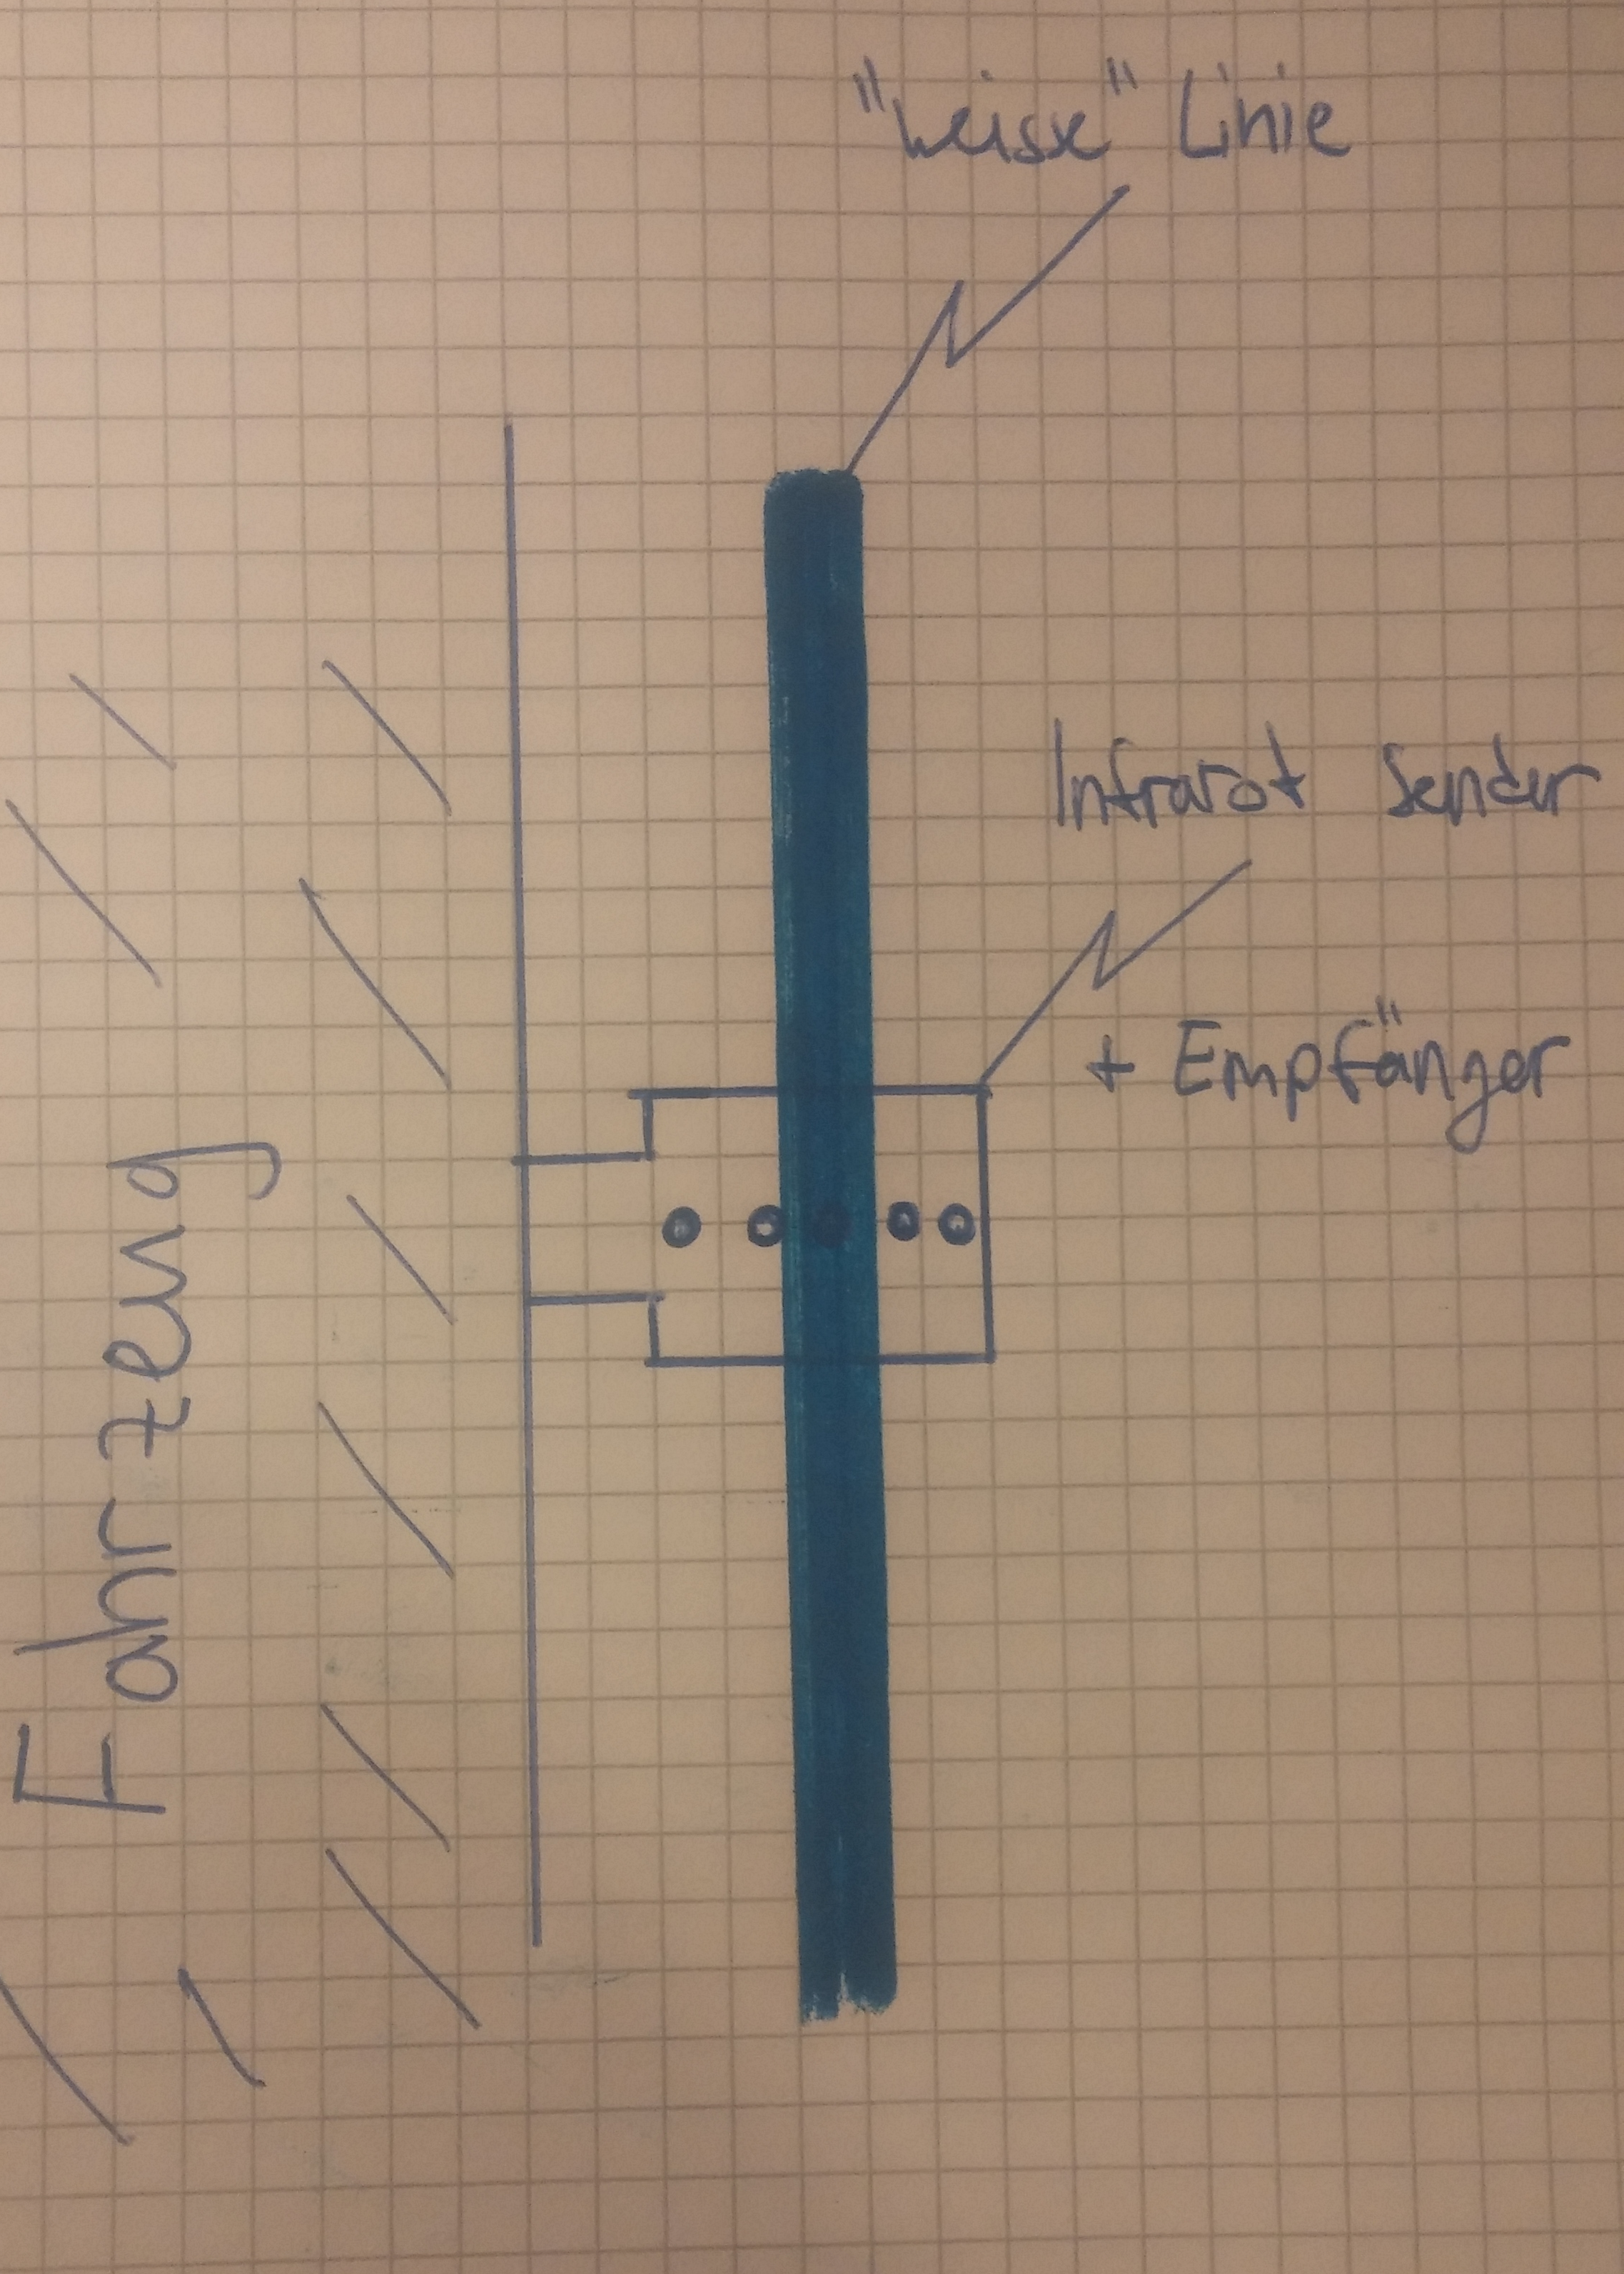
\includegraphics[width=\textwidth]{fig/Linienerkennung_1.png}
		\caption{1.Situation: Sensoren über der Linie}
	\end{subfigure}
	\hfill
	\begin{subfigure}[b]{0.36\textwidth}
		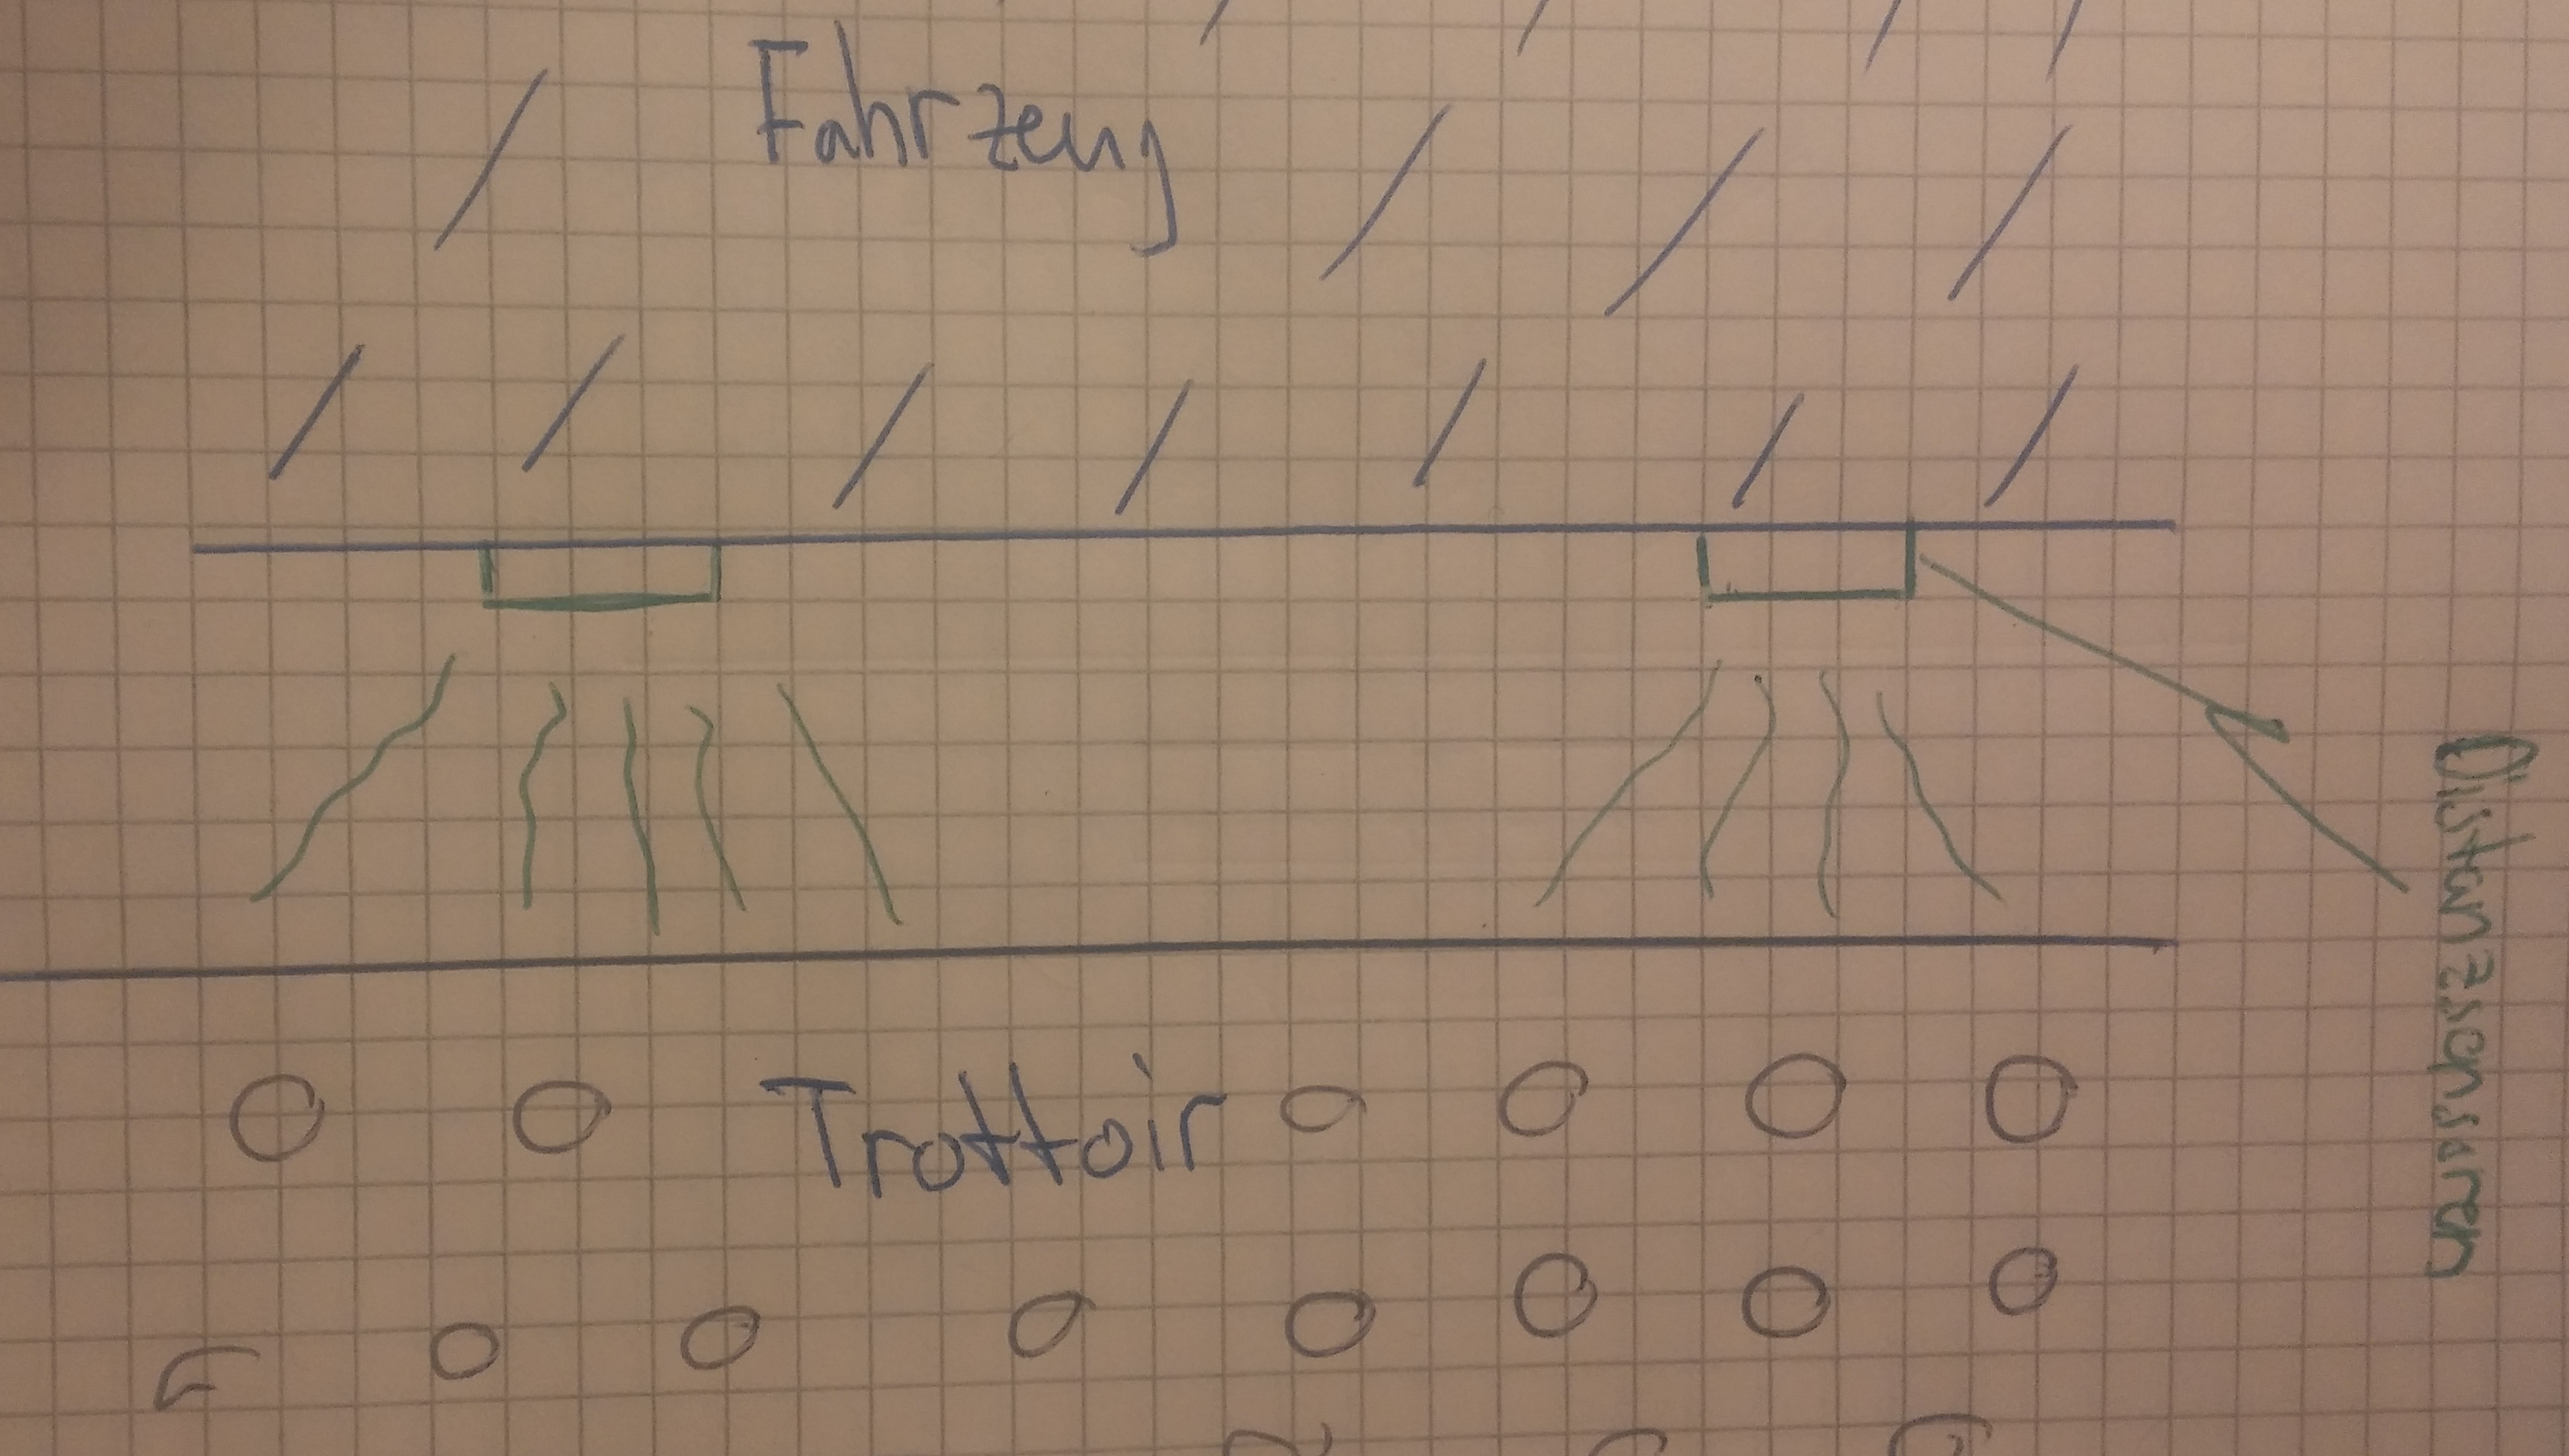
\includegraphics[width=\textwidth]{fig/Trottoirerkennung_1.png}
		\caption{2. Situation: Sensoren für die Abstandserkennung}
\end{subfigure}
	\caption{Mögliche Spurerkennung mit Distanzsensoren}\label{fig:animals}
\end{figure}



\begin{table}[h]
\begin{tabular}{p{0.5\textwidth} | p{0.5\textwidth}}


 \textbf{Vorteile} & \textbf{Nachteile} \\ \hline
	 
\begin{itemize}
\item Gut zu testen (Funktionsmuster)
\item Gute Präzision wird erwartet
\end{itemize}

 
 &
 
\begin{itemize}
\item Braucht externe Hardware und Verkabelung
\item Funktionsmuster zwingend notwendig
\end{itemize}

\end{tabular}
\end{table}

\begin{table}[h]
\begin{tabular}{p{0.5\textwidth}p{0.5\textwidth}}

 \textbf{Risiken} & \\ \hline
	 
\begin{itemize}
\item Die Linie lässt sich nicht Erkennen (ohne Konflikte mit der Anforderungsliste)
\item Das Trottoir ist zu wenig hoch damit es sich erkennen lässt
\end{itemize}
&
\begin{itemize}
\item Die Steuerung aufgrund der Linienerkennung ist nicht praktikabel
\end{itemize}

 
\end{tabular}
\end{table}

\pagebreak


%##############
\subsection{Bilderkennung}
Grafik

\begin{table}[h]
\begin{tabular}{p{0.5\textwidth} | p{0.5\textwidth}}


 \textbf{Vorteile} & \textbf{Nachteile} \\ \hline
	 
\begin{itemize}
\item Vorteil 1
\item Vorteil 2
\item Vorteil 3
\item ...
\end{itemize}

 
 &
 
\begin{itemize}
\item Nachteil 1
\item Nachteil 2
\item Nachteil 3
\item ...
\end{itemize}

\end{tabular}
\end{table}

\begin{table}[h]
\begin{tabular}{p{0.5\textwidth}p{0.5\textwidth}}


 \textbf{Risiken} & \\ \hline
	 
\begin{itemize}
\item Risiko 1
\item Risiko 2
\end{itemize}
&
\begin{itemize}
\item Risiko 3
\item ...
\end{itemize}

 
\end{tabular}
\end{table}

\pagebreak

% !TEX root = morphkasten.tex

\section{Containererkennung (grob)}


%##############
\subsection{Sensor}

\begin{figure} [hbp]
	\centering
	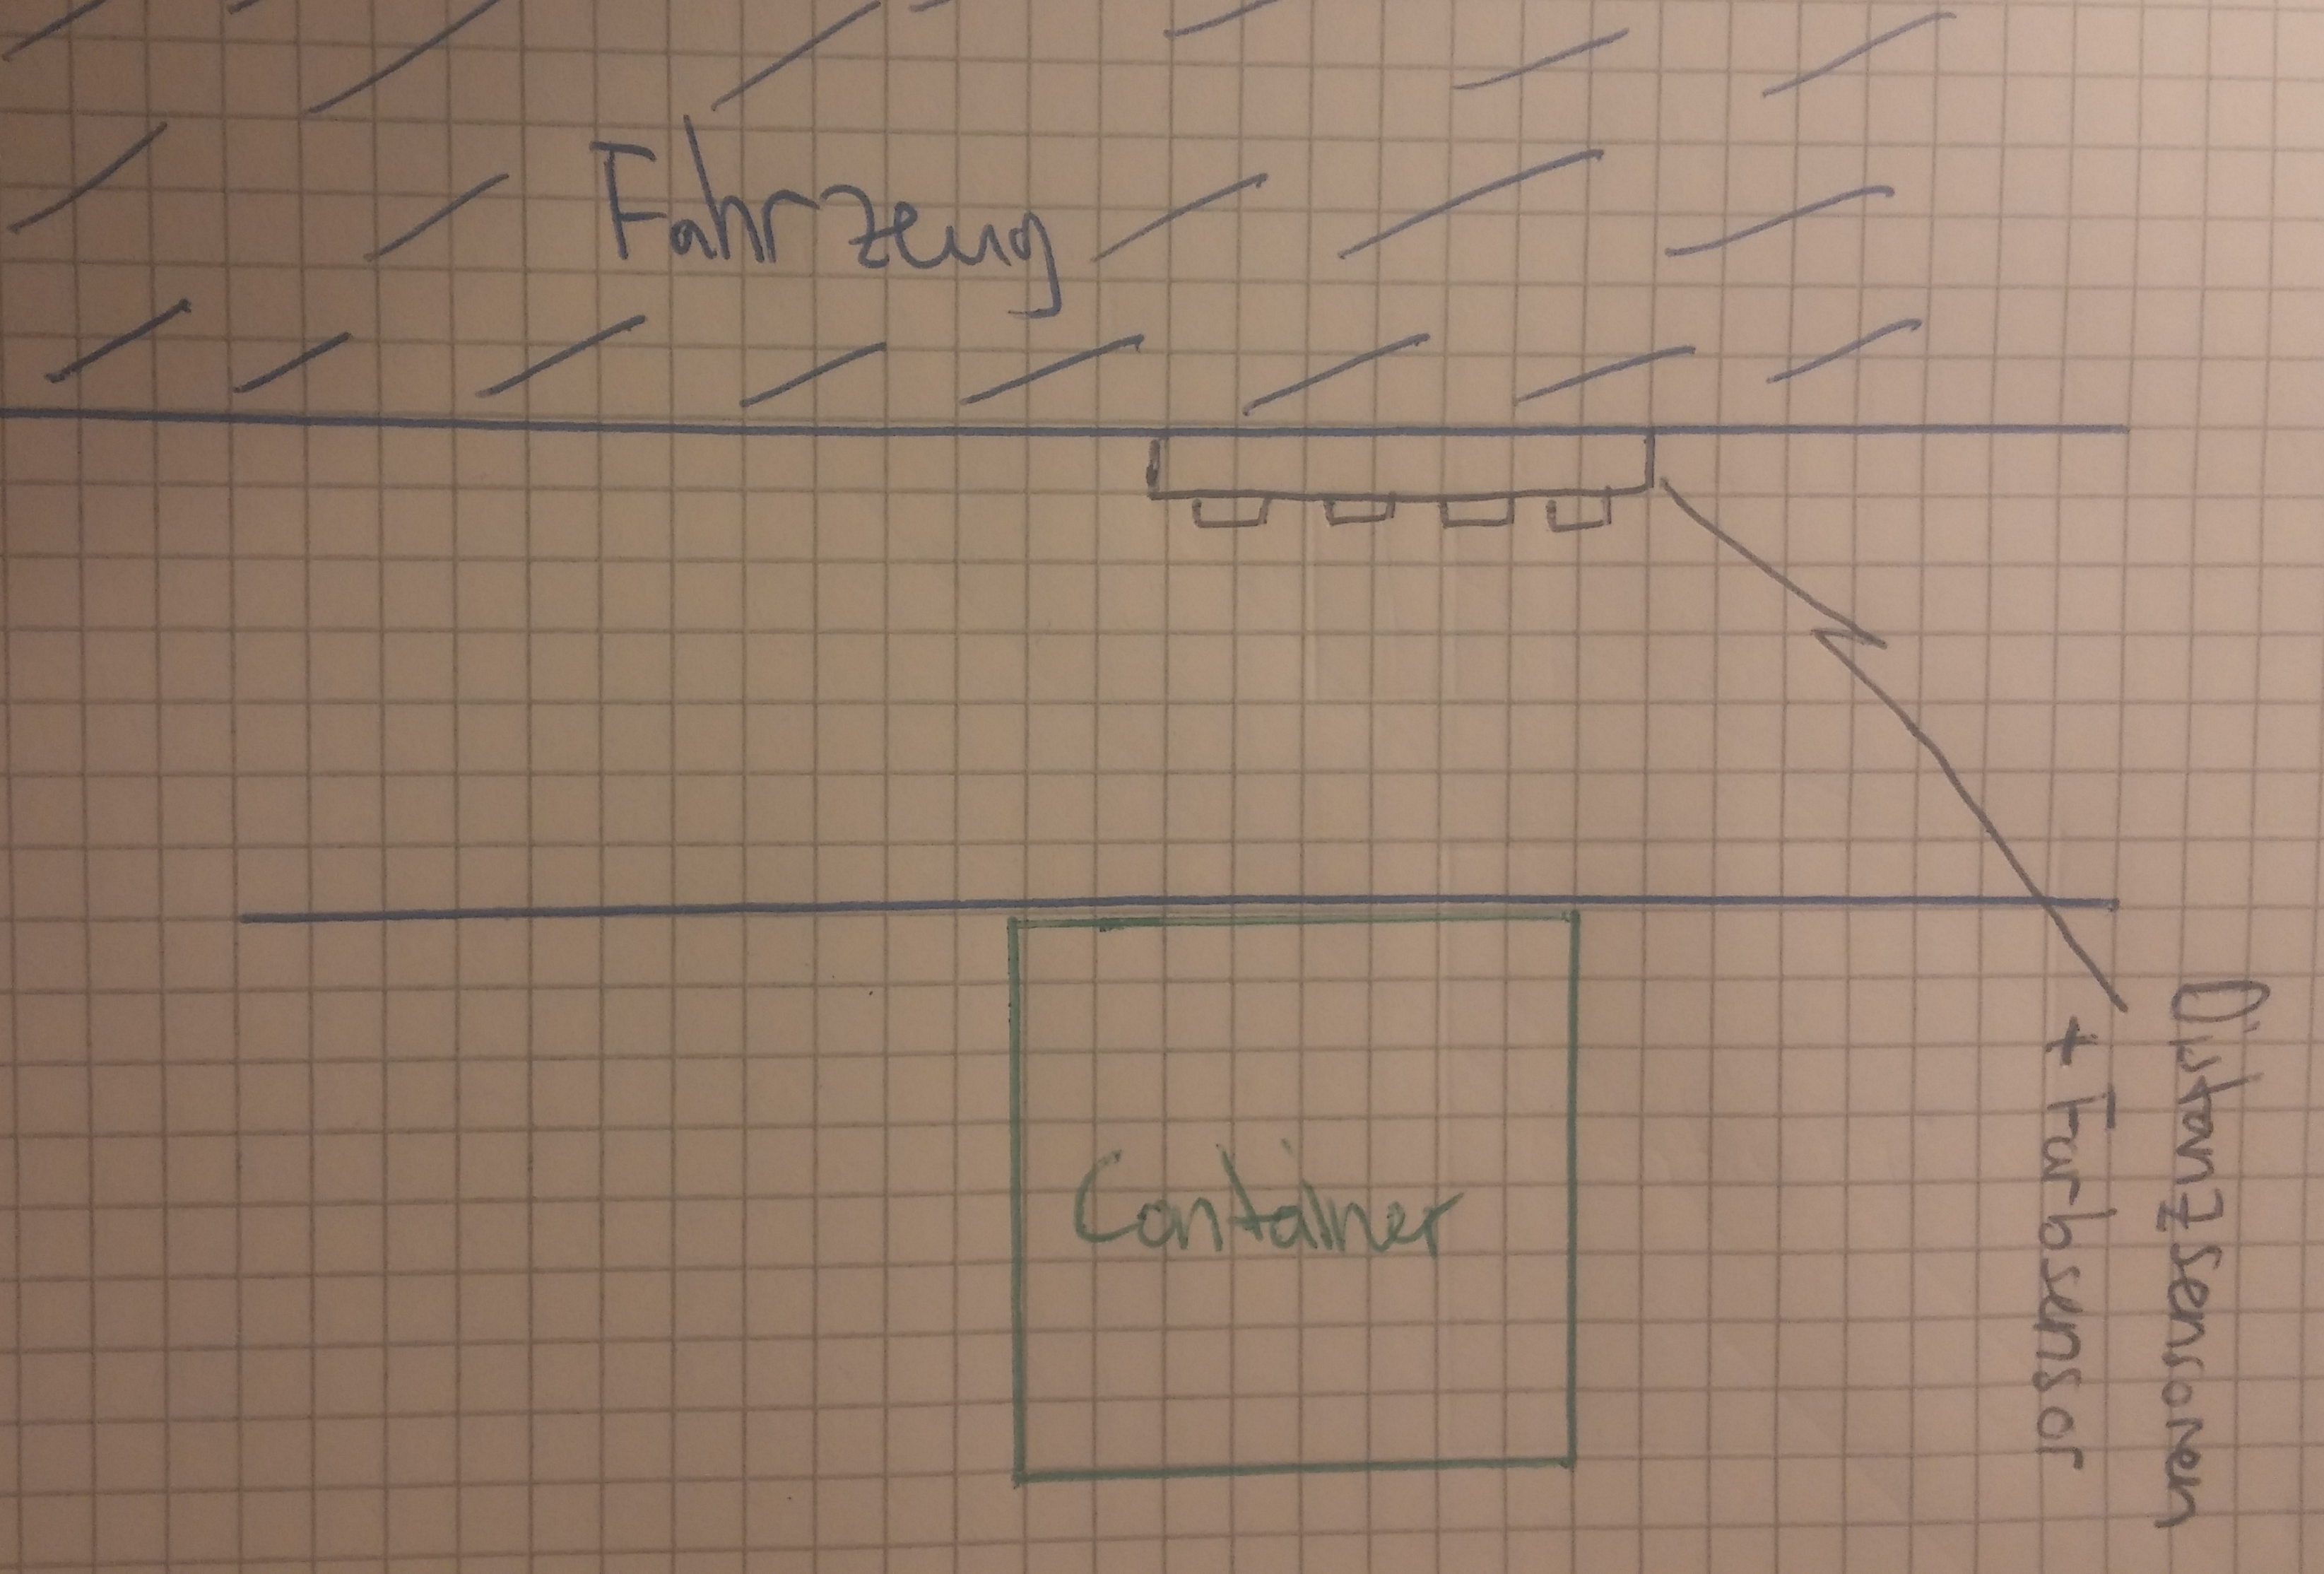
\includegraphics[width=0.5\textwidth]{fig/Containererkennung_2.png}
	\caption{Beispielhafte Containererkennung mit Sensoren}
\end{figure}

\begin{table}[h]
\begin{tabular}{p{0.5\textwidth} | p{0.5\textwidth}}


 \textbf{Vorteile} & \textbf{Nachteile} \\ \hline
	 
\begin{itemize}
\item Farberkennung möglich
\item Präzise Erkennung des Containers (wahrscheinlich)
\item Mehrfachverwendung mit anderen Anwendungen denkbar
\item Kostengünstig
\end{itemize}

 
 &
 
\begin{itemize}
\item Unbekannte Präzision
\item Je nach Sensor Störanfälligkeit
\item Zusatzhardware und Verkabelung nötig
\item 
\end{itemize}

\end{tabular}
\end{table}

\begin{table}[h]
\begin{tabular}{p{0.5\textwidth}p{0.5\textwidth}}


 \textbf{Risiken} & \\ \hline
	 
\begin{itemize}
\item Die Sensoren sind zu ungenau
\item Die Sensoren werden zu fest gestört
\end{itemize}
&
\begin{itemize}
\item Die Farbe kann auf Distanz nicht erkannt werden
\item Die Sensoren können zwischen Container und Sonstigem nicht unterscheiden
\end{itemize}

 
\end{tabular}
\end{table}

\pagebreak


%##############
\subsection{Bilderkennung}
\begin{figure}[h!]%Position festigen
\centering
\includegraphics[width=0.7\textwidth]{fig/containererkennung_grob_bilderkennung.png}
\caption{Bilderkennung Container}
\label{fig:Bilderkennung Container}
\end{figure}

\begin{table}[h]
\begin{tabular}{p{0.5\textwidth} | p{0.5\textwidth}}


\textbf{Vorteile} & \textbf{Nachteile} \\ \hline
	 
\begin{itemize}
\item bei grösserer Distanz zu Container schon erkennbar
\item Containererkennung durch Form- und/oder Farberkennung
\end{itemize}

 
 &
 
\begin{itemize}
\item Algorithmus nötig
\item rechenintensiv
\end{itemize}

\end{tabular}
\end{table}

\begin{table}[h]
\begin{tabular}{p{0.5\textwidth}p{0.5\textwidth}}

\textbf{Risiken} & \\ \hline
	 
\begin{itemize}
\item bei verschiedene Lichtverhätlnissen variieren die Farben
\item Container kann zum Teil von anderen Gegeständen verdeckt sein
\end{itemize}

 
\end{tabular}
\end{table}

\pagebreak

% !TEX root = morphkasten.tex

\section{Containererkennung (detailliert)}
Die Containererkennung muss auch ausgelegt sein für die Erkennung des Entladebehälters!

%##############
\subsection{Distanzsensor}
Die detaillierte Containererkennung mit Sensoren unterscheidet sich nur geringfügig von der groben Variante. Der Hauptunterschied besteht darin, dass bei der detaillierten Variante nur noch die Positionierung des Fahrzeugs vorzunehmen ist. Die Auswertung der Form und der Farbe wird Vorgängig von der Kamera erledigt und an das Mikrocontrollerboard weitergeleitet.
\begin{figure} [hbp]
	\centering
	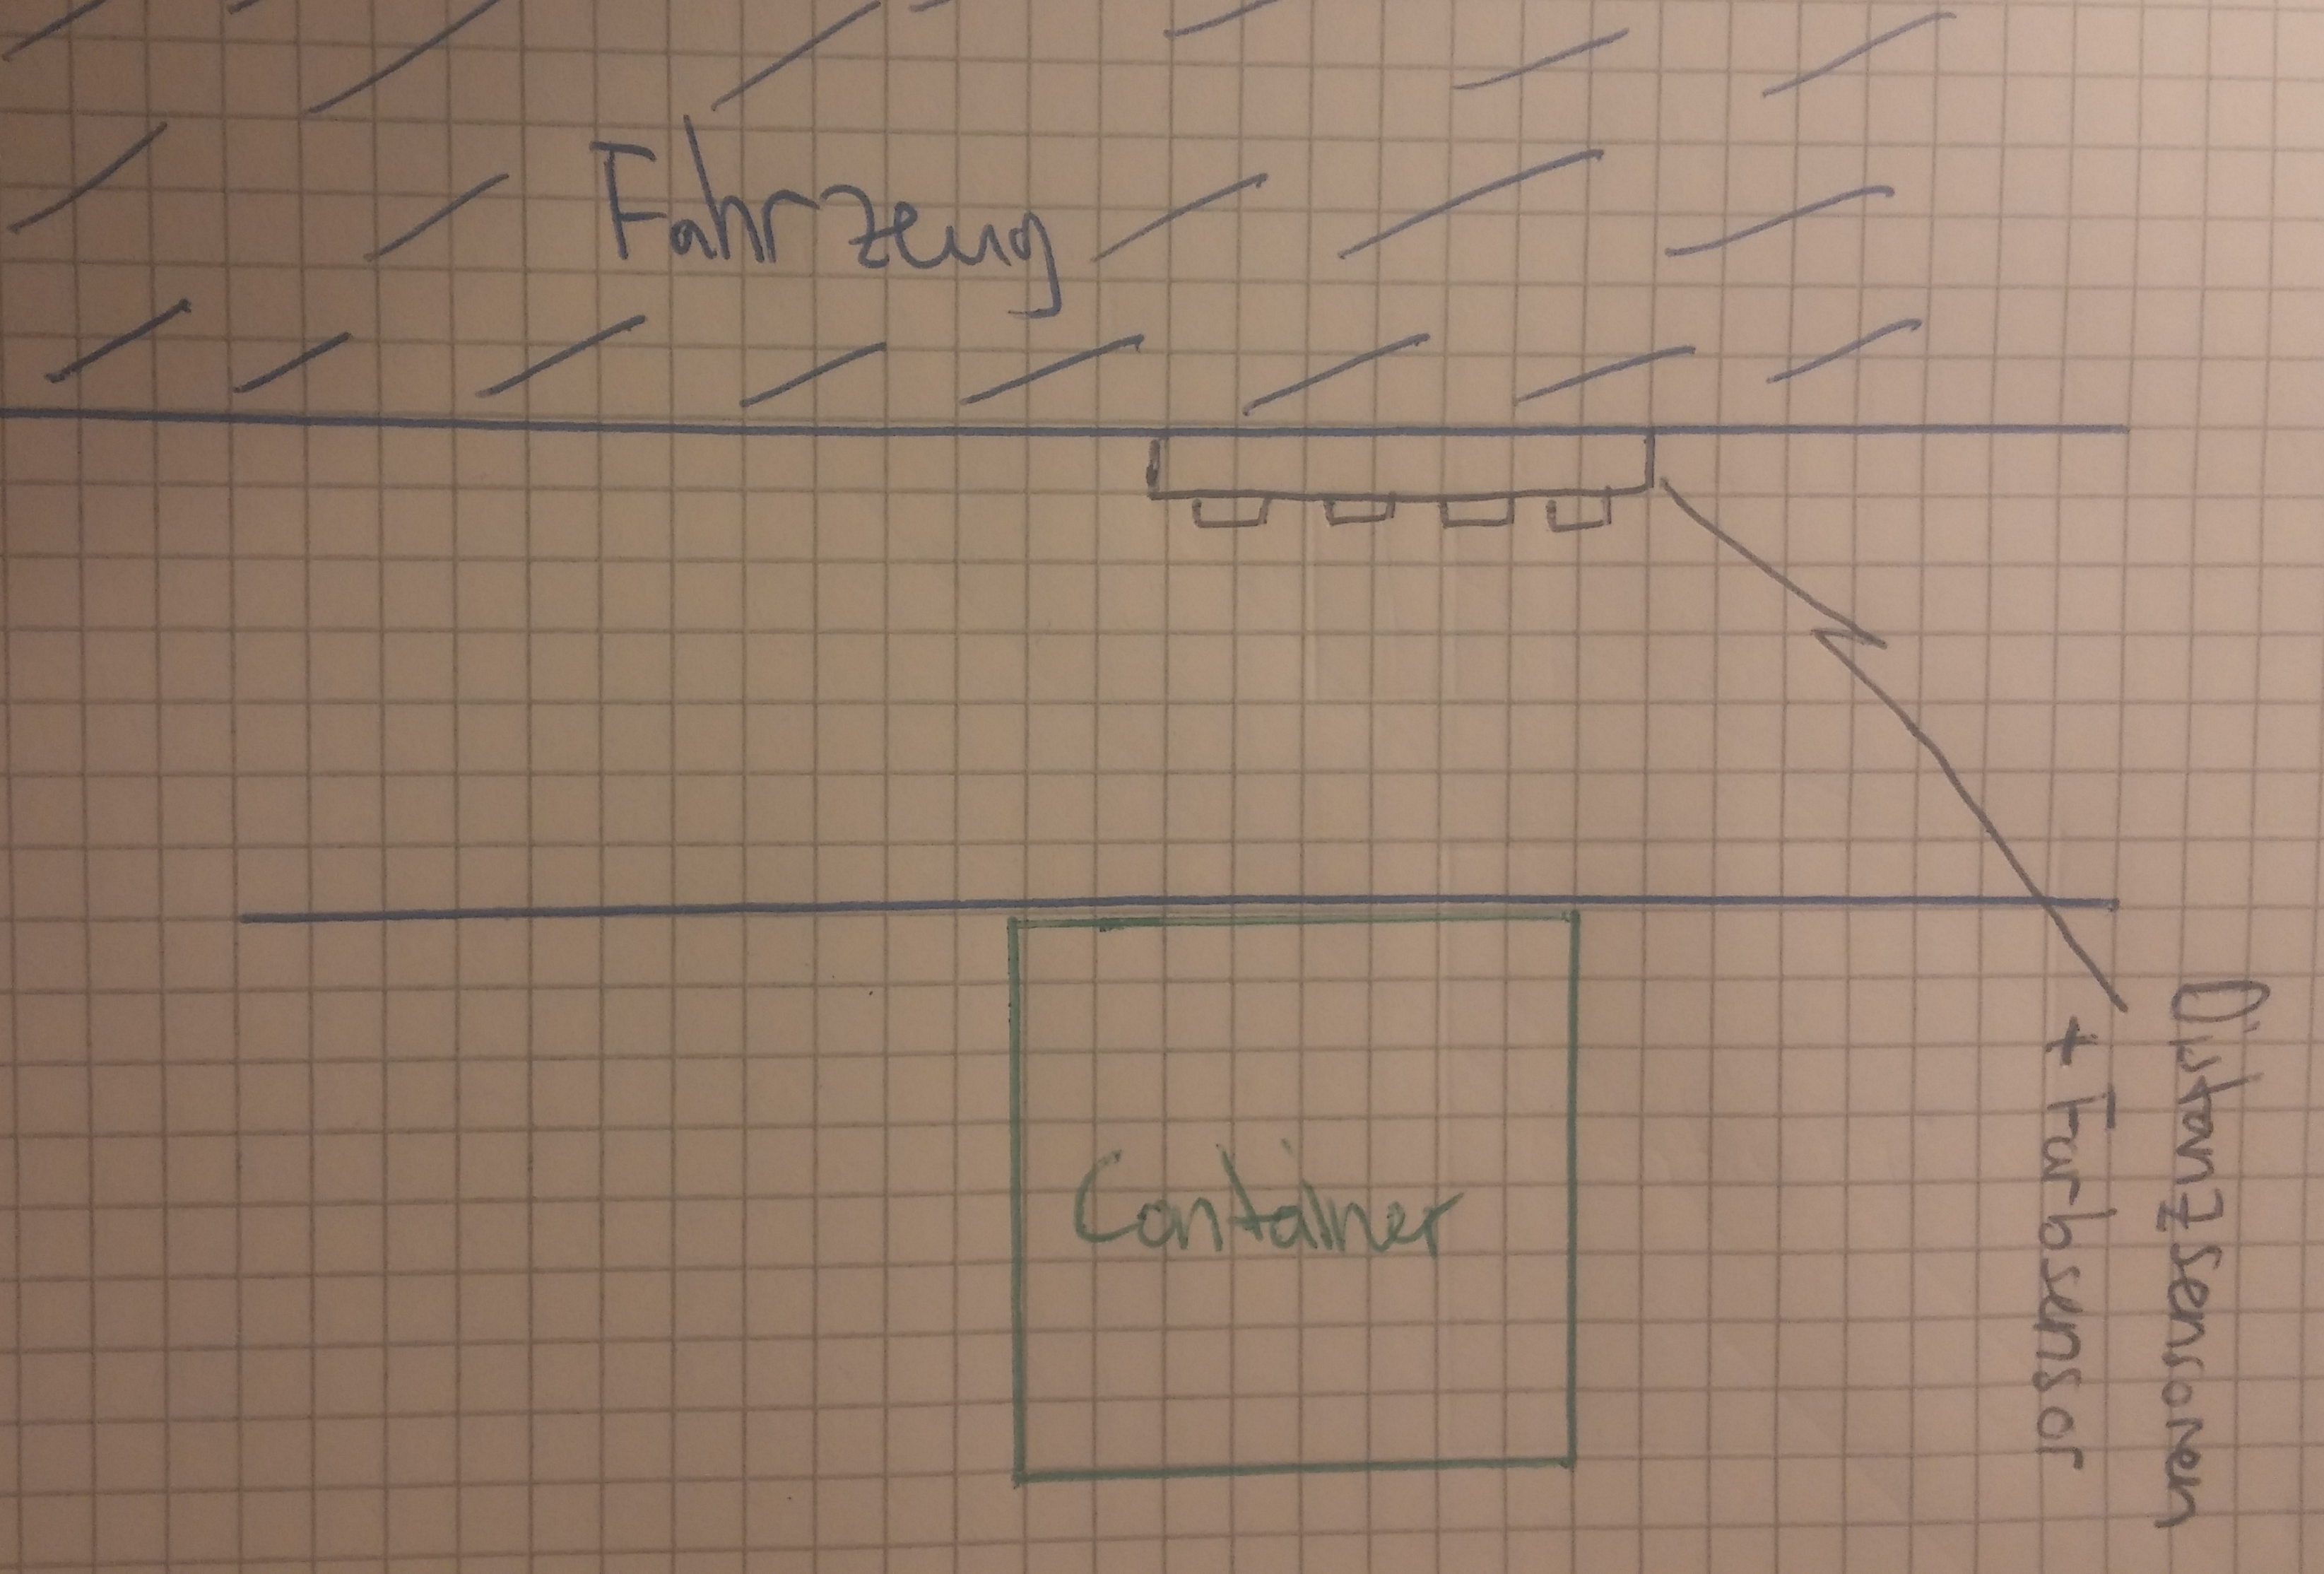
\includegraphics[width=0.5\textwidth]{fig/Containererkennung_2.png}
	\caption{Beispielhafte Containererkennung mit Distanzsensoren (ohne Farbsensor)}
\end{figure}

\begin{table}[h]
\begin{tabular}{p{0.5\textwidth} | p{0.5\textwidth}}


 \textbf{Vorteile} & \textbf{Nachteile} \\ \hline
	 
\begin{itemize}
\item Präzise Erkennung des Containers (wahrscheinlich)
\item Mehrfachverwendung mit anderen Anwendungen denkbar
\item Kostengünstig (kein Farbsensor)
\end{itemize}

 
 &
 
\begin{itemize}
\item Unbekannte Präzision
\item Je nach Sensor Störanfälligkeit
\item Zusatzhardware und Verkabelung nötig
\end{itemize}

\end{tabular}
\end{table}

\begin{table}[h]
\begin{tabular}{p{0.5\textwidth}p{0.5\textwidth}}


 \textbf{Risiken} & \\ \hline
	 
\begin{itemize}
\item Die Sensoren sind zu ungenau
\item Die Sensoren werden gestört

\end{itemize}
&
\begin{itemize}
\item Die Kommunikation der groben und detaillierten Erkennung ist zu langsam
\end{itemize}

 
\end{tabular}
\end{table}

\pagebreak


%##############
\subsection{Bilderkennung}
\begin{figure}[h!]%Position festigen
\centering
\includegraphics[width=0.7\textwidth]{fig/containererkennung_detailliert_bilderkennung.png}
\caption{Bilderkennung Container}
\label{fig:Bilderkennung Container}
\end{figure}
\begin{table}[h]
\begin{tabular}{p{0.5\textwidth} | p{0.5\textwidth}}


 \textbf{Vorteile} & \textbf{Nachteile} \\ \hline
	 
\begin{itemize}
\item Keine Sensoren zur Seite benötigt
\end{itemize}

 
 &
 
\begin{itemize}
\item Berechnung des Abstands muss auf wenige Milimeter stimmen
\item Keine Korrektur mehr möglich, wenn der Container aus dem Kamerbereich verschwindet
\end{itemize}

\end{tabular}
\end{table}

\begin{table}[h]
\begin{tabular}{p{0.5\textwidth}p{0.5\textwidth}}


 \textbf{Risiken} & \\ \hline
	 
\begin{itemize}
\item Ungenauigkeit bei der Distanzabschätzung
\item Container kann zum Teil von anderen Gegeständen verdeckt sein
\end{itemize}

 
\end{tabular}
\end{table}

\pagebreak


% !TEX root = morphkasten.tex

\section{Rechtsvortritt}


%##############
\subsection{Sensor}

Grafik

\begin{table}[h]
\begin{tabular}{p{0.5\textwidth} | p{0.5\textwidth}}


 \textbf{Vorteile} & \textbf{Nachteile} \\ \hline
	 
\begin{itemize}
\item Vorteil 1
\item Vorteil 2
\item Vorteil 3
\item ...
\end{itemize}

 
 &
 
\begin{itemize}
\item Nachteil 1
\item Nachteil 2
\item Nachteil 3
\item ...
\end{itemize}

\end{tabular}
\end{table}

\begin{table}[h]
\begin{tabular}{p{0.5\textwidth}p{0.5\textwidth}}


 \textbf{Risiken} & \\ \hline
	 
\begin{itemize}
\item Risiko 1
\item Risiko 2
\end{itemize}
&
\begin{itemize}
\item Risiko 3
\item ...
\end{itemize}

 
\end{tabular}
\end{table}

\pagebreak


%##############
\subsection{Bilderkennung}

\begin{figure}[h!]%Position festigen
\centering
\includegraphics[width=0.7\textwidth]{fig/rechtsvortritt_bilderkennung.png}
\caption{Bilderkennung Rechtsvortritt}
\label{fig:Bilderkennung Rechtsvortritt}
\end{figure}

\begin{table}[h]
\begin{tabular}{p{0.5\textwidth} | p{0.5\textwidth}}


 \textbf{Vorteile} & \textbf{Nachteile} \\ \hline
	 
\begin{itemize}
\item Stoppen durch Vorausplnung möglich
\item Unterschiede berechnen, wie sich das andere Fahrzeug bewegt
\end{itemize}

 
 &
 
\begin{itemize}
\item Genaue Definition, was ein Fahzeug an der Kreuzung beim Rechtsvortritt ist
\item rechenintensiv
\end{itemize}

\end{tabular}
\end{table}

\begin{table}[h]
\begin{tabular}{p{0.5\textwidth}p{0.5\textwidth}}


\textbf{Risiken} & \\ \hline
	 
\begin{itemize}
\item Fahrzeug wird auch an anderen Stellen erkennt
\item andere Gegenstände könnten als Fahrzeug interpretiert werden

\end{itemize}

 
\end{tabular}
\end{table}

\pagebreak

% !TEX root = morphkasten.tex

\section{Programmiersprache}


%##############
\subsection{Java}

\begin{figure}[h!]%Position festigen
\centering
\includegraphics[width=0.5\textwidth]{fig/java.jpeg}
\caption{Java (Quelle: http://www.t3n.de)}
\label{fig:Java}
\end{figure}

\begin{table}[h]
\begin{tabular}{p{0.5\textwidth} | p{0.5\textwidth}}


 \textbf{Vorteile} & \textbf{Nachteile} \\ \hline
	 
\begin{itemize}
\item Objektorientiert
\item Unterstützt Multithreading
\item Plattformunabhängig
\end{itemize}

 
 &
 
\begin{itemize}
\item Langsamer als C++
\end{itemize}

\end{tabular}
\end{table}

\begin{table}[h]
\begin{tabular}{p{0.5\textwidth}p{0.5\textwidth}}


 \textbf{Risiken} & \\ \hline
	 
\begin{itemize}
\item Bilderkennung könnte zu langsam sein
\end{itemize}

 
\end{tabular}
\end{table}

\pagebreak


%##############
\subsection{C++}
\begin{figure}[h!]%Position festigen
\centering
\includegraphics[width=0.5\textwidth]{fig/cplusplus.png}
\caption{C++ (Quelle: http://www.unixstickers.com)}
\label{fig:C++}
\end{figure}
\begin{table}[h]
\begin{tabular}{p{0.5\textwidth} | p{0.5\textwidth}}


 \textbf{Vorteile} & \textbf{Nachteile} \\ \hline
	 
\begin{itemize}
\item Objektorientiert
\item Schneller als Java
\item In den meisten Tutorials von OpenCV wird mit C++ programmiert
\item Unterstützt Multithreading
\end{itemize}

 
 &
 
\begin{itemize}
\item Komplexer als Java
\end{itemize}

\end{tabular}
\end{table}

\begin{table}[h]
\begin{tabular}{p{0.5\textwidth}p{0.5\textwidth}}


 \textbf{Risiken} & \\ \hline
	 
\begin{itemize}
\item Komplexität
\end{itemize}

 
\end{tabular}
\end{table}

\pagebreak

% !TEX root = morphkasten.tex

\section{Bilderkennungs-Bibliothek}


%##############
\subsection{OpenCV}

\begin{figure}[h!]%Position festigen
\centering
\includegraphics[width=0.3\textwidth]{fig/opencv.png}
\caption{OpenCV (Quelle: https://en.wikipedia.org/wiki/OpenCV)}
\label{fig:OpenCV}
\end{figure}

\begin{table}[h]
\begin{tabular}{p{0.5\textwidth} | p{0.5\textwidth}}



 \textbf{Vorteile} & \textbf{Nachteile} \\ \hline
	 
\begin{itemize}
\item Grosse Community
\item Läuft auf Linux
\item Kostenlos
\item Kompatibel mit Java und C++
\end{itemize}

 
 &
 
\begin{itemize}
\item Enthält auch viele Funktionen, welche nicht benötigt werden (komplex)
\end{itemize}

\end{tabular}
\end{table}

\begin{table}[h]
\begin{tabular}{p{0.5\textwidth}p{0.5\textwidth}}


 \textbf{Risiken} & \\ \hline
	 
\begin{itemize}
\item Ressourcenknappheit
\end{itemize}

 
\end{tabular}
\end{table}

\pagebreak


%##############
\subsection{SimpleCV}
\begin{figure}[h!]%Position festigen
\centering
\includegraphics[width=0.5\textwidth]{fig/simplecv.png}
\caption{SimpleCV (Quelle: http://google-opensource.blogspot.ch/2012\_08\_01\_archive.html)}
\label{fig:SimpleCV}
\end{figure}

\begin{table}[h]
\begin{tabular}{p{0.5\textwidth} | p{0.5\textwidth}}


 \textbf{Vorteile} & \textbf{Nachteile} \\ \hline
	 
\begin{itemize}
\item Läuft auf Linux
\item Freie Software
\item Kompatibel mit Java und C++
\end{itemize}

 &
 
\begin{itemize}
\item Community kleiner als bei OpenCV
\end{itemize}

\end{tabular}
\end{table}

\begin{table}[h]
\begin{tabular}{p{0.5\textwidth}p{0.5\textwidth}}


\textbf{Risiken} & \\ \hline
	 
\begin{itemize}
\item Zu Problemen wird keine Lösung gefunden
\item Ressourcenknappheit
\end{itemize}
 
\end{tabular}
\end{table}

\pagebreak

% !TEX root = morphkasten.tex
\section{Anhang}
% !TEX root = morphkasten.tex


%##############
\subsection{Farbsensor}
\begin{figure}[h]
	\centering
	\includegraphics[width=0.5\textwidth]{fig/Farbsensor}
	\caption{Freedomboard KL25 von Freescale (Quelle: www.miniinthebox.com)}
	%http://miniimg1.rightinthebox.com/images/384x384/201310/bvlklo1383018315288.jpg
\end{figure}


\begin{table}[h]
\begin{tabular}{p{0.5\textwidth} | p{0.5\textwidth}}


 \textbf{Vorteile} & \textbf{Nachteile} \\ \hline
	 
\begin{itemize}
\item Im Preisrahmen, ein Farbsensor kostet ungefähr 10.-
\end{itemize}

 &
 
\begin{itemize}
\item Benötigt  AD Eingänge
\item Distanz abhängig
\end{itemize}

\end{tabular}
\end{table}

\begin{table}[h]
\begin{tabular}{p{0.5\textwidth}p{0.5\textwidth}}


 \textbf{Risiken} & \\ \hline
	 
\begin{itemize}
\item Distanz hat zu grossen Einfluss auf die Farberkennung
\item Die Farben lassen sich nicht zuverlässig erkennen (Sensorseite)
\end{itemize}
&
\begin{itemize}
\item Die Auswertung ist sehr aufwändig (Mikrocontrollerseitig)
\end{itemize}

 
\end{tabular}
\end{table}

\pagebreak


%##############
\subsection{Ultraschallsensoren}
\begin{figure}[h]
	\centering
	\includegraphics[width=0.5\textwidth]{fig/ultraschallsensor.png}
	\caption{Beispielhaftes Tinkerforge System (Bricks mit Ultraschallmodul) (Quelle: www.generationrobots.com)}
	%http://www.generationrobots.com/2653-large_default/ultraschallsensor-hc-sr04.jpg
\end{figure}

\begin{table}[h]
\begin{tabular}{p{0.5\textwidth} | p{0.5\textwidth}}


\textbf{Vorteile} & \textbf{Nachteile} \\ \hline
	 
\begin{itemize}
\item Erschwinglich, ein Sensor kostet ungefähr 5.Fr
\item Unempfindlich auf Störeinflüsse (Ausser andere Ultraschallsensoren)
\item Grosse Distanz (>10cm)
\end{itemize}
 &
\begin{itemize}
\item Kann nicht als als Liniensensor eingesetzt werden
\item Keine klaren Grenzen (relativ grosser Abstrahlwinkel)
\end{itemize}
\end{tabular}
\end{table}


\begin{table}[h]
\begin{tabular}{p{0.5\textwidth}p{0.5\textwidth}}


 \textbf{Risiken} & \\ \hline
	 
\begin{itemize}
\item Andere Ultraschallsensoren stören die Messung
\item Der Bereich ist zu ungenau
\end{itemize}
&
\begin{itemize}
\item Die Anbindung funktioniert nicht richtig
\end{itemize}

 
\end{tabular}
\end{table}

\pagebreak

%##############
\subsection{Infrarotsensoren}
\begin{figure}[h]
	\centering
	\includegraphics[width=0.5\textwidth]{fig/Infrarotsensor.jpg}
	\caption{Infrarotsensor (Quelle: www.tinkerforge.com)}
	%https://www.tinkerforge.com/de/shop/media/catalog/product/cache/2/image/600x600/9df78eab33525d08d6e5fb8d27136e95/s/e/sensor_gp2y0a21yk0f_tilted_600.jpg
\end{figure}
%http://www.farnell.com/datasheets/1725394.pdf

\begin{table}[h]
\begin{tabular}{p{0.5\textwidth} | p{0.5\textwidth}}


\textbf{Vorteile} & \textbf{Nachteile} \\ \hline
	 
\begin{itemize}
\item Kostengünstig (Sensor und Empfänger kosten zusammen 1.7Fr)
\item Kann als Liniensensor und Rad-Encoder eingesetzt werden.
\item Eher klaren Grenzen (kleiner Abstrahlwinkel)
\end{itemize}
 &
\begin{itemize}
\item Benötigt zwei AD Eingänge
\item Sind empfindlich auf UV-Licht
\item Geringe Reichweite (je nach Typ nur bis 5mm)
\item Als Liniensensor: Nicht senkrechtes Abtasten ist problematisch
\end{itemize}
\end{tabular}
\end{table}


\begin{table}[h]
\begin{tabular}{p{0.5\textwidth}p{0.5\textwidth}}


 \textbf{Risiken} & \\ \hline
	 
\begin{itemize}
\item Die Sensoren werden gestört
\item Die Sensoren sind zu ungenau
\end{itemize}
&
\begin{itemize}
\item Die Anbindung funktioniert nicht richtig
\end{itemize}

 
\end{tabular}
\end{table}

\pagebreak

\end{document}